
\documentclass{article} % Especially this!

\usepackage[english]{babel}
\usepackage[utf8]{inputenc}
\usepackage[margin=1.5in]{geometry}
\usepackage{amsmath}
\usepackage{amsthm}
\usepackage{amsfonts}
\usepackage{amssymb}
\usepackage[usenames,dvipsnames]{xcolor}
\usepackage{graphicx}
\usepackage[siunitx]{circuitikz}
\usepackage{tikz}
\usepackage[colorinlistoftodos, color=orange!50]{todonotes}
\usepackage{hyperref}
\usepackage[numbers, square]{natbib}
\usepackage{fancybox}
\usepackage{epsfig}
\usepackage{soul}
\usepackage[framemethod=tikz]{mdframed}
\usepackage[shortlabels]{enumitem}
\usepackage[version=4]{mhchem}
\usepackage{listings}
\usepackage{epstopdf}


\epstopdfDeclareGraphicsRule{.gif}{png}{.png}{convert gif:#1 png:\OutputFile}
\AppendGraphicsExtensions{.gif}






%%%%%%%%%%%%%%%%%%%%%%%%%%%%%%%%%%%%%%%%%%%%%%%%%%%%%%%%%
%  _______ ______          _____ _    _ ______ _____  	%
% |__   __|  ____|   /\   / ____| |  | |  ____|  __ \ 	%
%    | |  | |__     /  \ | |    | |__| | |__  | |__) |	%
%    | |  |  __|   / /\ \| |    |  __  |  __| |  _  / 	%
%    | |  | |____ / ____ \ |____| |  | | |____| | \ \ 	%
%    |_|  |______/_/    \_\_____|_|  |_|______|_|  \_\	%
%%%%%%%%%%%%%%%%%%%%%%%%%%%%%%%%%%%%%%%%%%%%%%%%%%%%%%%%%
%														%
% 			COMMANDS				SUMMARY				%
% \clarity{points}{comment} >>> "Clarity of Writing"	%
% \other{points}{comment}	>>> "Other"					%
% \spelling{comment}		>>> "Spelling"				%
% \units{comment}			>>> "Units"					%
% \english{comment}			>>> "Syntax and Grammer"	%
% \source{comment}			>>> "Sources"				%
% \concept{comment}			>>> "Concept"				%
% \missing{comment}			>>> "Missing Content"		%
% \maths{comment}			>>> "Math"					%
% \terms{comment}			>>> "Science Terms"			%
%														%
%%%%%%%%%%%%%%%%%%%%%%%%%%%%%%%%%%%%%%%%%%%%%%%%%%%%%%%%%
\setlength{\marginparwidth}{3.4cm}


% NEW COUNTERS
\newcounter{points}
\setcounter{points}{100}
\newcounter{spelling}
\newcounter{english}
\newcounter{units}
\newcounter{other}
\newcounter{source}
\newcounter{concept}
\newcounter{missing}
\newcounter{math}
\newcounter{terms}
\newcounter{clarity}

% COMMANDS

\definecolor{myblue}{rgb}{0.668, 0.805, 0.929}
\newcommand{\hlb}[2][myblue]{ {\sethlcolor{#1} \hl{#2}} }

\newcommand{\clarity}[2]{\todo[color=CornflowerBlue!50]{CLARITY of WRITING(#1) #2}\addtocounter{points}{#1}
\addtocounter{clarity}{#1}}

\newcommand{\other}[2]{\todo{OTHER(#1) #2} \addtocounter{points}{#1} \addtocounter{other}{#1}}

\newcommand{\spelling}{\todo[color=CornflowerBlue!50]{SPELLING (-1)} \addtocounter{points}{-1}
\addtocounter{spelling}{-1}}
\newcommand{\units}{\todo{UNITS (-1)} \addtocounter{points}{-1}
\addtocounter{units}{-1}}

\newcommand{\english}{\todo[color=CornflowerBlue!50]{SYNTAX and GRAMMAR (-1)} \addtocounter{points}{-1}
\addtocounter{english}{-1}}

\newcommand{\source}{\todo{SOURCE(S) (-2)} \addtocounter{points}{-2}
\addtocounter{source}{-2}}
\newcommand{\concept}{\todo{CONCEPT (-2)} \addtocounter{points}{-2}
\addtocounter{concept}{-2}}

\newcommand{\missing}[2]{\todo{MISSING CONTENT (#1) #2} \addtocounter{points}{#1}
\addtocounter{missing}{#1}}

\newcommand{\maths}{\todo{MATH (-1)} \addtocounter{points}{-1}
\addtocounter{math}{-1}}
\newcommand{\terms}{\todo[color=CornflowerBlue!50]{SCIENCE TERMS (-1)} \addtocounter{points}{-1}
\addtocounter{terms}{-1}}


\newcommand{\summary}[1]{
\begin{mdframed}[nobreak=true]
\begin{minipage}{\textwidth}
\vspace{0.5cm}
\begin{center}
\Large{Grade Summary} \hrule 
\end{center} \vspace{0.5cm}
General Comments: #1

\vspace{0.5cm}
Possible Points \dotfill 100 \\
Points Lost (Science Terms) \dotfill \theterms \\
Points Lost (Syntax and Grammar) \dotfill \theenglish \\
Points Lost (Spelling) \dotfill \thespelling \\
Points Lost (Units) \dotfill \theunits \\
Points Lost (Math) \dotfill \themath \\
Points Lost (Sources) \dotfill \thesource \\
Points Lost (Concept) \dotfill \theconcept \\
Points Lost (Missing Content) \dotfill \themissing \\
Points Lost (Clarity of Writing) \dotfill \theclarity \\
Other \dotfill \theother \\[0.5cm]
\begin{center}
\large{\textbf{Grade:} \fbox{\thepoints}}
\end{center}
\end{minipage}
\end{mdframed}}

%#########################################################

%To use symbols for footnotes
\renewcommand*{\thefootnote}{\fnsymbol{footnote}}
%To change footnotes back to numbers uncomment the following line
%\renewcommand*{\thefootnote}{\arabic{footnote}}

% Enable this command to adjust line spacing for inline math equations.
% \everymath{\displaystyle}


%title
\title{
\normalfont \normalsize 
\textsc{Indian Institute of Technology Bombay \\ 
CS684 Autumn Semester 2016} \\
[10pt] 
\rule{\linewidth}{0.5pt} \\[6pt] 
\huge Interrupts and Timers\\
\rule{\linewidth}{2pt}  \\[10pt]
}
\author{E.R.T.S. Lab}
\date{\normalsize \today}

\begin{document}

\maketitle
\noindent

%lab Objective
\section{Lab Objective}
% Yada Yada Yada
This lab will introduce you to the use of Timers and Interrupts on the TM4C123GH6PM.

\section{Pre-requisite}
\begin{enumerate}
\item 
Lab 1: Interface led and both the switches.
\item Reference material: Please go through \href{https://www.cse.iitb.ac.in/~erts/html_pages/Resources/Tiva/TM4C123G_LaunchPad_Workshop_Workbook.pdf}{\textbf{Resources7-Chapter 4}} before you proceed further.

\end{enumerate}


%%% Problem Statement
\section{Problem Statement}

% Materials go here
%%%%%%%%%%%%%%%%%%%%%%%
% FOR A NUMBERED LIST
% \begin{enumerate}
% \item Your_Item
% \end{enumerate}
%%%%%%%%%%%%%%%%%%%%%%%
% FOR A BULLETED LIST
% \begin{itemize}
% \item Your_Item
% \end{itemize}
%%%%%%%%%%%%%%%%%%%%%%%
\begin{enumerate}
\item 
Use sw1 to change the color of the led (R$\Rightarrow$ G$\Rightarrow$ B$\Rightarrow$ R….) where you should press the switch just once instead of long press in Lab 1. Use switch debouncing mentioned below in the procedure to differentiate between switch bounce and actual key press.
\item
Use sw2 to increment a global variable once for each button press. Check if the variable always increments by one (adjust the time interval of 10 ms if you wish to)
\end{enumerate}





%Relevant Theory
\newpage
\section {Relevant Theory}
%%%%%%%%%%%%%%%%%%%%%%%
% FOR A NUMBERED LIST
% \begin{enumerate}
% \item Your_Item
% \end{enumerate}
%%%%%%%%%%%%%%%%%%%%%%%

This lab will use a timer to generate interrupts and we will write a timer interrupt service routine (ISR) that implements a state machine to perform \textbf{“software button debouncing”}.
\begin{figure}
\centering
\includegraphics[scale=0.8]{buttonBounce.gif}
\caption{Button Bounce Waveform}
\footnote{Image courtesy: $https://students.cs.byu.edu/~cs224ta/references/HowTos/HowTo_Interrupts.php$}
\end{figure}
\\
\\
\textbf{Button Bounce:}From the above diagram it is clear that when you press the switch the signal bounces for a finite amount of time before settling down to its final logic state. This is due to the tendency of any two metal contacts in an electronic device to generate multiple signals as the contacts close or open. The bounce period is ~10 to 20 ms. 
\\
\\
\textbf{Solution: }There are several ways to do button debouncing which includes modifications in both hardware and software. In this lab we will explore software debouncing. In software debouncing too, there are a couple of ways to solve this problem viz. 
\begin{enumerate}
\item  \textbf{Polling the switch plus introducing finite delays:} 
In polling method the controller is busy polling the switch hence it will not be able to perform any other tasks.
\item \textbf{Using interrupts and timers:} If we want to use this time to do other tasks, then we can use interrupts and timers. \\ 
\end{enumerate}
\textbf{Switch debouncing using interrupts and timers:} We will check for the status of the switch at finite intervals (say 10 ms). This time interval will be generated using timers. When the 10 ms interval is over the timer should generate an interrupt and the code in the interrupt service routine (ISR) will be executed. In the interrupt service routine, we will implement a state machine. Here the idea is that if we find the switch pressed for two successive intervals (of 10 ms) then we confirm that the switch is pressed and we will detect the next key press only if we confirm that the switch is released. This will ensure that if a switch press is only detected once. 

A state machine is described below for implementing software debouncing. 
\begin{figure}
\centering
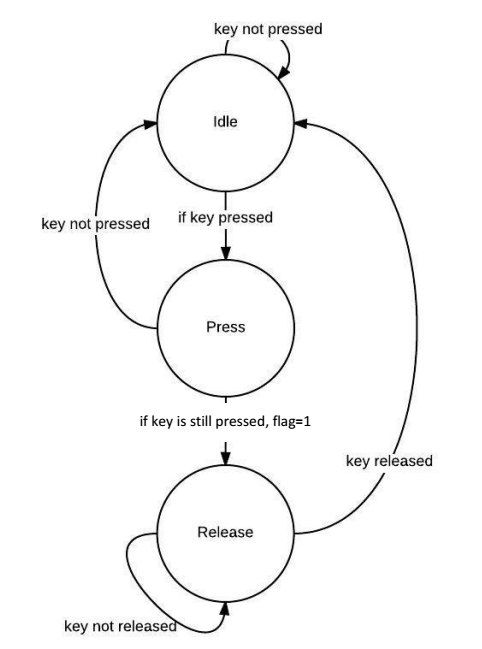
\includegraphics[scale=0.8]{stateChart.png}
\caption{Switch debouncing state diagram}
\label{sm}
\end{figure}
In this state machine there are three states viz. Idle, Press and Release for a switch.
There are two transition paths in each state. Any state transition condition is checked after a fixed interval
of time which is set by a timer (in this case it is 10 ms).
\\
\textbf{Note:} As the bounce period is ~10 ms to 20 ms you can change this time interval based on your experimental
trials. It is possible that different switches have different bounce periods.
\\
\\
\textbf{IDLE} \\
If the key is pressed, enter press state\\
else remain in IDLE state
\\
\\
\textbf{PRESS} \\
If key is still pressed, then enter release state and make flag 1 indicating that key was pressed.\\
else return to idle state (de-bouncing period)
\\
\\
\textbf{RELEASE} \\
If the key is released, then enter an idle state\\
else remain in release state until key is released.
\newpage
%%%Procedure
%%%%%%%%%%%%%%%%%%%%%%%%%%%%%%
\section {Procedure}
%%%%%%%%%%%%%%%%%%%%%%%%%%%%%%
% TO IMPORT AN IMAGE
% UPLOAD IT FIRST (HIT THE PROJECT BUTTON TO SHOW FILES)
% KEEP THE NAME SHORT WITH NO SPACES!
% TYPE THE FOLLOWING WITH THE NAME OF YOUR FILE
% DON'T INCLUDE THE FILE EXTENSION
% \includegraphics[width=\textwidth]{name_of_file}
% \textwidth makes the picture the width of the paragraphs
%%%%%%%%%%%%%%%%%%%%%%%%%%%%%%
% TO CREATE A FIGURE WITH A NUMBER AND CAPTION
% \begin{figure}
% \includegraphics[width=\textwidth]{image}
% \caption{Your Caption Goes Here}
% \label{your_label}
% \end{figure}
% REFER TO YOUR FIGURE LATER WITH
% \ref{your_label}
% LABELS NEED TO BE ONE WORD
%%%%%%%%%%%%%%%%%%%%%%%%%%%%%
\begin{enumerate}
\item 
Configure and initialize Timer 0 and set the time interval to 10ms. Use the lab exercise in \href{https://www.cse.iitb.ac.in/~erts/html_pages/Resources/Tiva/TM4C123G_LaunchPad_Workshop_Workbook.pdf}{\textbf{Resources7-Chapter 4}} as a starting point.
\item
Make a user defined function called “detectKeyPress ()” and call this in the interrupt handler. This function will return 1 only if a key press is detected according to the state machine.
The prototype of the function is given below.
\begin{verbatim}
unsigned char detectKeyPress()
{
return flag;
}
\end{verbatim}
\item
Describe the state machine\textbf{Figure:\ref{sm}} in this function and each time the function is called from the interrupt handler the machine should make a transition to the next stage. Make sure that the previous state (Scope of variables) of the system is maintained each time the function is called.
\item
Write a code for debouncing both sw1 and sw2.
\item
Verify that both the switches are debounced.
\item
Show the output to your TA and explain if you were able to complete the problem statement.
\end{enumerate}





%%% Demo and Submissions
\section {Demo and Submissions}
%%%%%%%%%%%%%%%%%%%%%%%%%%%%%%%%%%%%%%%%%%%%%%%%
You have to shoot two individual videos demonstrating the output of the problem statement.
Your codes for each of the problem statement has to be uploaded in Github repository.








%\subsection{Definitions}
% Include your sources!
%%%%%%%%%%%%%%%%%%%%%%%
% LIST OF DEFINITIONS
% \begin{description}
% \item [WORD] {Definition}
% \end{description}
%%%%%%%%%%%%%%%%%%%%%%%






%\subsection{Results}
% State your main discovery based on the experimental data.






%\subsection{Questions}
% Write full question and format answers in ITALIC
% CTRL + I for ITALIC











%  _____  ____  _    _ _____   _____ ______  _____ 
% / ____|/ __ \| |  | |  __ \ / ____|  ____|/ ____|
%| (___ | |  | | |  | | |__) | |    | |__  | (___  
% \___ \| |  | | |  | |  _  /| |    |  __|  \___ \ 
% ____) | |__| | |__| | | \ \| |____| |____ ____) |
%|_____/ \____/ \____/|_|  \_\\_____|______|_____/ 
%%%%%%%%%%%%%%%%%%%%%%%%%%%%%%%%%%%%%%%%%%%%%%%%%%%%


% USE NOCITE TO ADD SOURCES TO THE BIBLIOGRAPHY WITHOUT SPECIFICALLY CITING THEM IN THE DOCUMENT

%\nocite{ref_num}


%%%%%%%%%%%%%%%%%%%%%%%%%%%%%%%%%%%%%%%%%%%%%%%%%%%%%%

			% BIBLIOGRAPHY: %

% Make sure your class *.bib file is uploaded to this project by clicking the project button > add files. Change 'sample' below to the name of your file without the .bib extension.
%%%%%%%%%%%%%%%%%%%%%%%%%%%%%%%%%%%%%%%%%%%%%%%%%%

%\bibliographystyle{plainnat}
%\bibliography{sample}

% UNCOMMENT THE TWO LINES ABOVE TO ENABLE BIBLIOGRAPHY

%%%%%%%%%%%%%%%%%%%%%%%%%%%%%%%%%%%%%%%%%%%%%%%%%%


\end{document} % NOTHING AFTER THIS LINE IS PART OF THE DOCUMENT
